% Standalone XeLaTeX source; standard commands and distributed packages only.
% Source: public/notes/物工/問題/2022ap_exam.pdf, PDF pp. 4--5.
\documentclass[11pt,a4paper]{article}
\usepackage[margin=24mm]{geometry}
\usepackage{fontspec}
\usepackage{xeCJK}
\setCJKmainfont{HaranoAjiMincho-Regular.otf}
\setCJKsansfont{HaranoAjiGothic-Medium.otf}
\usepackage{amsmath,amssymb}
\usepackage{tikz}
\setlength{\parindent}{1em}
\setlength{\parskip}{0.35em}
\title{物理工学専攻 院試解答集 ver2\\2022年 物理学 第2問}
\author{政岡凜太郎}
\date{}
\begin{document}
\maketitle

図の幾何では $y$ は下向き正で、棒の方向単位ベクトルは $(\sin\theta,\cos\theta)$ である。振動する支点の変位は鉛直成分だけに加わる。
\begin{center}
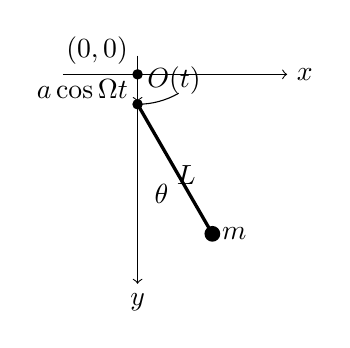
\begin{tikzpicture}[scale=0.95]
% Illustration parameters at t=0: theta=30 degrees, a/L=0.20.
\def\L{2.0}
\def\amp{0.4}
\def\ang{30}
\pgfmathsetmacro{\px}{\L*sin(\ang)}
\pgfmathsetmacro{\py}{-(\amp+\L*cos(\ang))}
\draw[->] (-1.0,0)--(2.0,0) node[right] {$x$};
\draw[->] (0,0.25)--(0,-2.8) node[below] {$y$};
\fill (0,0) circle (2pt) node[above left] {$(0,0)$};
\fill (0,-\amp) circle (2pt) node[above right] {$O(t)$};
\draw[densely dashed] (0,0)--(0,-2.35);
\draw[->] (0,-0.03)--(0,{-\amp+0.03}) node[midway,left] {$a\cos\Omega t$};
\draw[very thick] (0,-\amp)--(\px,\py);
\fill (\px,\py) circle (3pt) node[right] {$m$};
\draw (0,-\amp) arc[start angle=270,end angle={270+\ang},radius=0.55*\L];
\pgfmathsetmacro{\arcx}{0.62*\L*cos(285)}
\pgfmathsetmacro{\arcy}{-\amp+0.62*\L*sin(285)}
\node at (\arcx,\arcy) {$\theta$};
\node at ({0.55*\px+0.10},{-\amp+0.55*(\py+\amp)}) {$L$};
\end{tikzpicture}
\end{center}

\section*{[1] おもりの座標}
支点からおもりへの変位は $(L\sin\theta,L\cos\theta)$ なので
\[
\boxed{x=L\sin\theta,\qquad y=a\cos\Omega t+L\cos\theta}.
\]

\section*{[2] Cartesian の運動方程式}
張力は支点へ向かうため $x$ 成分は $-T\sin\theta$、下向き $y$ 成分は $-T\cos\theta$。重力は下向き正だから
\[
\boxed{m\ddot x=-T\sin\theta,\qquad m\ddot y=mg-T\cos\theta}.
\]

\section*{[3] 座標の二階微分}
[1] を時間微分すると
\[
\boxed{\ddot x=L(\ddot\theta\cos\theta-\dot\theta^2\sin\theta)},\qquad
\boxed{\ddot y=-a\Omega^2\cos\Omega t-L(\ddot\theta\sin\theta+\dot\theta^2\cos\theta)}.
\]

\section*{[4] 張力を消去した角運動方程式}
第一式に $\cos\theta$ を掛け、第二式に $-\sin\theta$ を掛けて加えると張力が消え、
\[
m(\ddot x\cos\theta-\ddot y\sin\theta)=-mg\sin\theta.
\]
[3] の加速度を代入すると $\ddot x\cos\theta-\ddot y\sin\theta=L\ddot\theta+a\Omega^2\cos\Omega t\sin\theta$ なので
\[
\boxed{\ddot\theta+\frac{a\Omega^2}{L}\cos\Omega t\sin\theta=-\frac{g}{L}\sin\theta}.
\]

\section*{[5] 支点が静止したときの小振動}
微小角では $\sin\theta\simeq\theta$。$a=0$ の方程式は
\[
\ddot\theta_0+\frac gL\theta_0=0,\qquad \omega_0=\sqrt{\frac gL}.
\]
初期条件 $\theta_0(0)=A$, $\dot\theta_0(0)=0$ より
\[
\boxed{\theta_0(t)=A\cos\omega_0t}.
\]

\section*{[6] 振幅 $a$ の一次応答}
小角の方程式を $\theta=\theta_0+a\theta_1$ として展開する。$a^0$ の項は [5] の式、$a^1$ の項は
\[
\ddot\theta_1+\omega_0^2\theta_1=-\frac{\Omega^2}{L}\theta_0(t)\cos\Omega t
=-\frac{A\Omega^2}{2L}\left\{\cos[(\Omega+\omega_0)t]+\cos[(\Omega-\omega_0)t]\right\}.
\]
右辺には積和公式による二つの側帯波が現れる。

\section*{[7] 二つの側帯波をもつ特解}
特解 $\theta_1=u_1\cos[(\Omega+\omega_0)t]+u_2\cos[(\Omega-\omega_0)t]$ を [6] に代入する。各周波数の係数条件は
\[
\left[\omega_0^2-(\Omega+\omega_0)^2\right]u_1=-\frac{A\Omega^2}{2L},\qquad
\left[\omega_0^2-(\Omega-\omega_0)^2\right]u_2=-\frac{A\Omega^2}{2L}.
\]
$\Omega>0$ なので第1の分母は零にならず、第2の分母が零となるのは $\Omega=2\omega_0$ のときである。$A\ne0$ のとき、有限な二側帯波特解が存在する条件は
\[
\boxed{\Omega\ne2\sqrt{\frac gL}}.
\]
そのとき
\[
\boxed{u_1=\frac{A\Omega}{2L\left(\Omega+2\sqrt{g/L}\right)},\qquad
u_2=\frac{A\Omega}{2L\left(\Omega-2\sqrt{g/L}\right)}}.
\]
共鳴点 $\Omega=2\omega_0$ では差周波側帯波が固有振動と一致し、通常は永年項を含むためこの有界な形の特解は得られない。$A=0$ なら一次の駆動自体がなく、$\theta_1=0$ は共鳴点でも解である。
\end{document}
